\chapter{Fill Reducing Reorderings}
\label{app:app-fill-reducing-reodering}



%\figpointer{\ref{fig:mumps-ordering-3}}
\begin{figure}[!t]
\centering
	\begin{tabular}{cc}
		\subfloat[torso3]{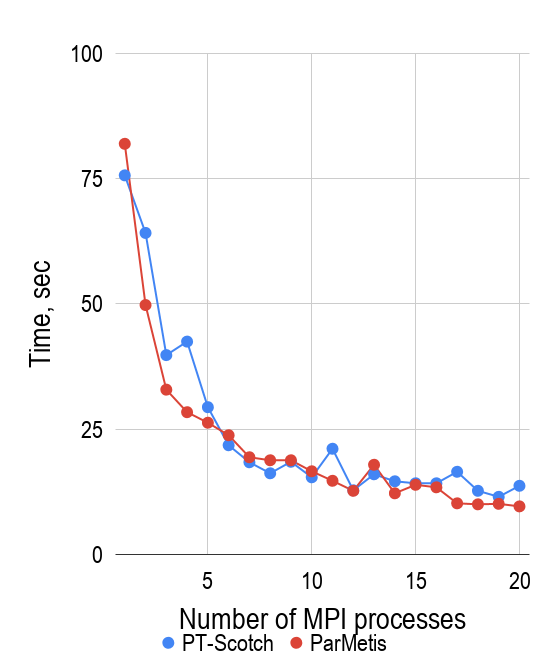
\includegraphics[width=0.48\textwidth]{figures/chapter-2/ordering/torso3.png}} &
		\subfloat[consph]{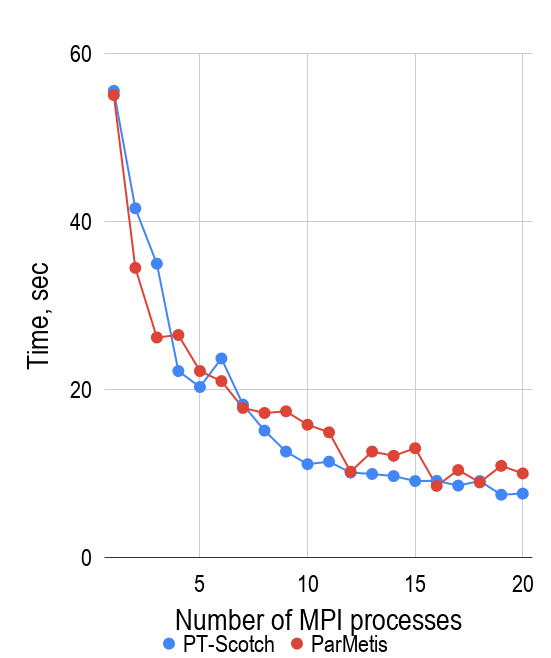
\includegraphics[width=0.48\textwidth]{figures/chapter-2/ordering/consph.png}} \\
		\subfloat[CurlCurl\_3]{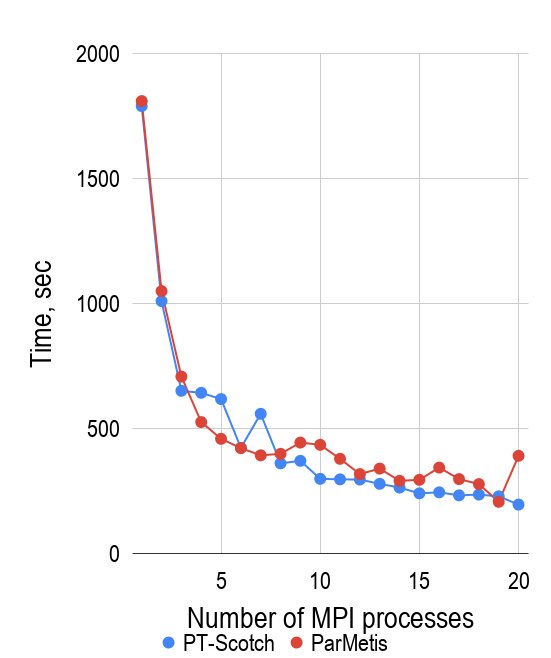
\includegraphics[width=0.48\textwidth]{figures/chapter-2/ordering/CurlCurl_3.png}} &
		\subfloat[x104]{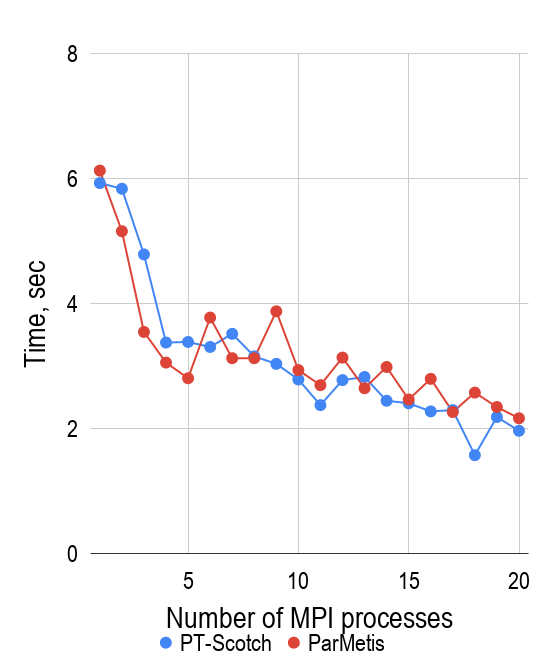
\includegraphics[width=0.48\textwidth]{figures/chapter-2/ordering/x104.png}} \\
	\end{tabular}
	\caption{An influence of different fill reducing algorithms on parallel factorizations of \textit{torso3}, \textit{consph}, \textit{CurlCurl\_3} and \textit{x104} matrices}
	\label{fig:mumps-ordering-3}
\end{figure}



%\figpointer{\ref{fig:mumps-ordering-4}}
\begin{figure}[!t]
\centering
	\begin{tabular}{cc}
		\subfloat[cant]{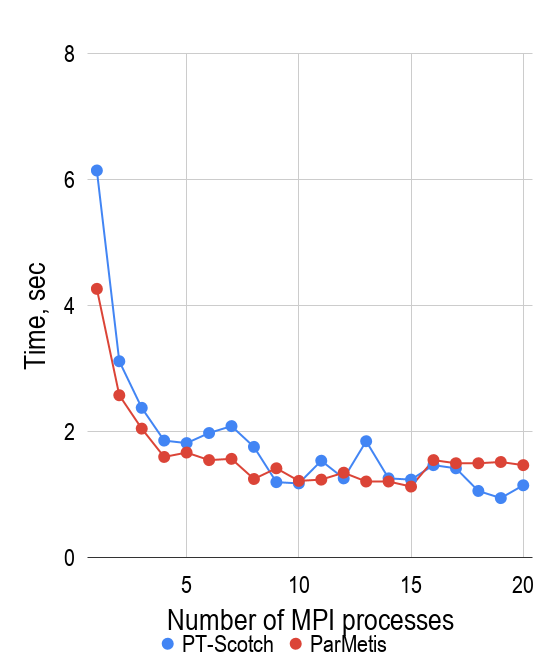
\includegraphics[width=0.48\textwidth]{figures/chapter-2/ordering/cant.png}} &
		\subfloat[memchip]{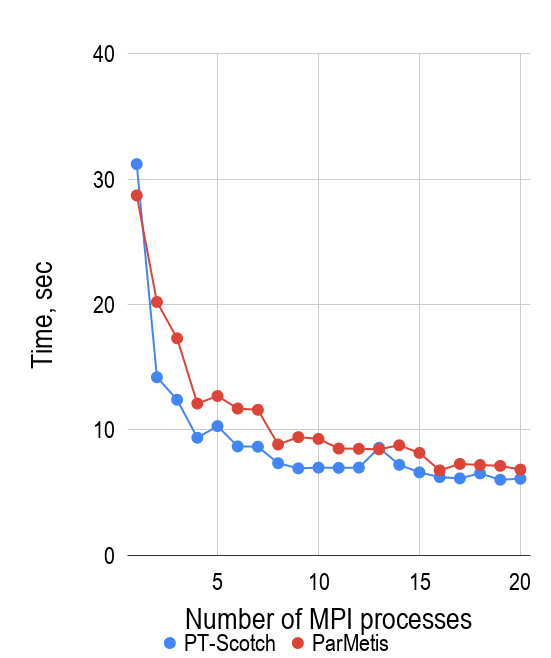
\includegraphics[width=0.48\textwidth]{figures/chapter-2/ordering/memchip.png}} \\
	\end{tabular}
	\caption{An influence of different fill reducing algorithms on parallel factorizations of \textit{cant} and \textit{memchip} matrices}
	\label{fig:mumps-ordering-4}
\end{figure}

